%
% Chapter 9
%

\chapter{SIGNAL EXTRACTION}
Despite the event selection being aimed at selecting signal and rejecting background, the signal region yields are dominated by background events,
and lack sufficient statistics to identify the presence of the \tth signal in data. These post-selection (pre-fit) yields are in Table~\ref{tab:yields} below.
Becuse the post-selection yields offer no discernable way of separating the signal in the data, additional discrimination is necessary. A multivariate strategy
relying on Boosted Decision Trees (BDTs) is used to further discriminate the \tth signal from various backgrounds. 

\begin{table}[htbp]
\begin{center}
  \caption[Signal region event yields by lepton flavor]{Expected (pre-fit) yields for signal and background processes, and observed yields in data. Uncertainties shown
are purely statistical.}
    \begin{tabular}{l c c c} \hline
& $\mu\mu$ & $ee$ & $e\mu$  \\ \hline 
$t\bar{t}W$ & 45.4 $\pm$ 0.5 & 17.8 $\pm$ 0.3 & 64.3 $\pm$ 0.6 \\
$t\bar{t}Z/\gamma^{*}$ & 16.8 $\pm$ 0.7 & 14.8 $\pm$ 0.8 & 41.7 $\pm$ 1.4 \\
\hline
WZ & 5.2 $\pm$ 0.7 & 1.6 $\pm$ 0.4 & 7.5 $\pm$ 0.8 \\
Rare SM. bkg & 6.8 $\pm$ 0.3 & 3.5 $\pm$ 0.2 & 11.7 $\pm$ 0.4 \\
WWss & 2.9 $\pm$ 0.2 & 1.4 $\pm$ 0.1 & 4.3 $\pm$ 0.2 \\
\hline
Conversions & 0.0 $\pm$ 0.0 & 3.4 $\pm$ 1.1 & 8.5 $\pm$ 1.3 \\
Charge flip & 0.0 $\pm$ 0.0 & 172 $\pm$ 93 & 149 $\pm$ 82 \\
Non-prompt leptons & 29.9 $\pm$ 1.2 & 17.3 $\pm$ 1.1 & 53.5 $\pm$ 1.8 \\
\hline
Total bkg & 107.3 $\pm$ 1.7 & 70.3 $\pm$ 1.8 & 208.0 $\pm$ 2.9 \\
 \hline
$t\bar{t}H$ & 18.5 $\pm$ 0.2 & 7.4 $\pm$ 0.1 & 26.2 $\pm$ 0.2 \\
 \hline
Data & 154 & 95 & 274 \\
\hline
\end{tabular}
    \label{tab:yields}
\end{center}
\end{table}

The signal extraction strategy adopted here targets the two largest backgrounds, \ttv and the non-prompt leptons, and uses BDTs to discriminate against each separately.
The inputs to these BDTs include event kinematics, as well as outputs of other BDTs, designed to resconstruct parts of the signal events such as the Higgs jets and the
hadronically decaying top quark. Finally, the outputs of the BDT dscriminators are binned in a uniqe approach which produces a final shape template that is used
for the final results.

\section{Two Dimensional BDTs}
Two BDTs are used to produce the final shape template. One BDT is trained exclusively against the \ttv background, while the other targets the background due to non-prompt
leptons. Because the non-prompt background is a data-driven estimation, all of the events making up this background cannot be used for MVA training, since the BDT must be
trained on a completely separate set of events from the set it is evaluated on. Because a large part of the fake background is comprised of the \ttbar process, the BDT is
trained against \ttbar MC. The outputs of the two BDTs are plotted on separate axes forming a two-dimensional shape. This two-dimensional shape is binned into rectangles
and the contents of which form a one-dimensional histogram. 

A loosened version of the $2lss$ signal region selection is applied to the training events. This loosened selection is motivated by increasing the training statistics available
while not affecting the behavior and kinematics of the input variables with respect to the signal region. This loosened selection consists of the following criteria:
\begin{itemize}
\item At least two preselected same-sign leptons
\item The lepton \pt $>$ 25,15 
\item At least 4 preselected jets among which there must be $\geq$ 2 CSVv2 L or $\geq$ 1 CSVv2 M
\end{itemize}

The input variables are selected considering not only the best individual separation power, but also the set that offers the best discrimination power of the BDT. These two
properties are not necessarily the same, since correlations and anti-correlations among varibles can differ substantially between signal and background, providing significant
discrimination power. Additionally, the closure between MC and data, also known as modeling, was considered since variables that are not modeled well in MC cannot be used to
approximate the variable's behavior in data. The input variables used for the BDT training against \ttbar include:
\begin{itemize}
\item the absolute value of the maximum psuedorapidity of the two leptons
\item the multiplicity of hadronic jets
\item the minimum angular distance between the leading lepton and the nearest jet
\item the minimum angular distance between the trailing lepton and the nearest jet
\item the transverse mass of the leading lepton and missing transverse energy
%\item the hadronic top reconstruction score
\end{itemize} 

\noindent the input variables used for the BDT training against \ttv include:
\begin{itemize}
\item the absolute value of the maximum psuedorapidity of the two leptons
\item the multiplicity of hadronic jets
\item the minimum angular distance between the leading lepton and the nearest jet
\item the minimum angular distance between the trailing lepton and the nearest jet
\item the transverse mass of the leading lepton and missing transverse energy
\item the leading lepton transverse momentum
\item the trailing lepton transverse momentum
\item the Higgs jet tagger score after hadronic top removal
\end{itemize} 

\noindent The discrimination power of these input variables against the largest backgrounds is available in Figures~\ref{fig:inputs1}~\ref{fig:inputs2}~\ref{fig:inputs3}.
The reconstruction inputs offer improved discrimination power against both of the largest backgrounds, see Figure~\ref{fig:inputs3}.

\begin{figure}[htp]
\centering
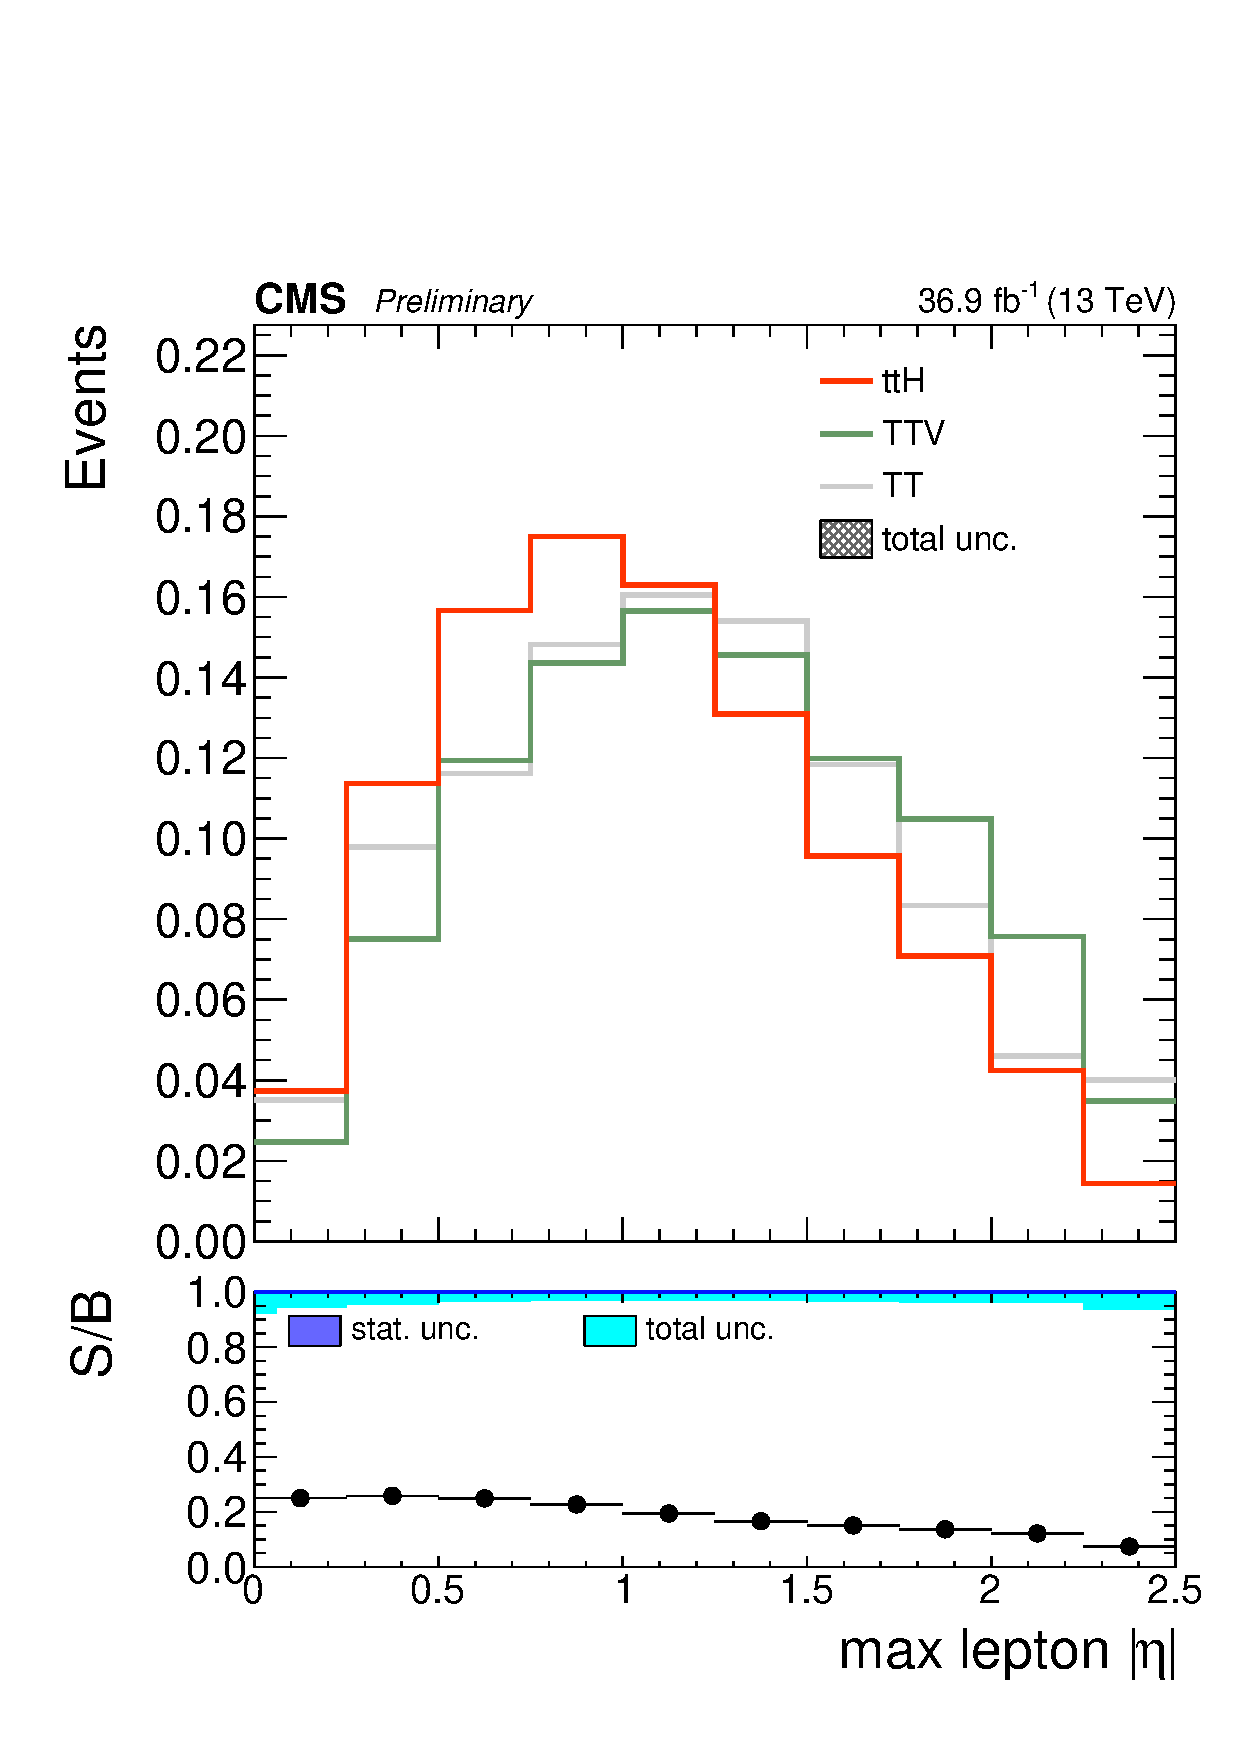
\includegraphics[width=0.49\textwidth]{ch9_figs/kinMVA_input_max_Lep_eta.pdf}
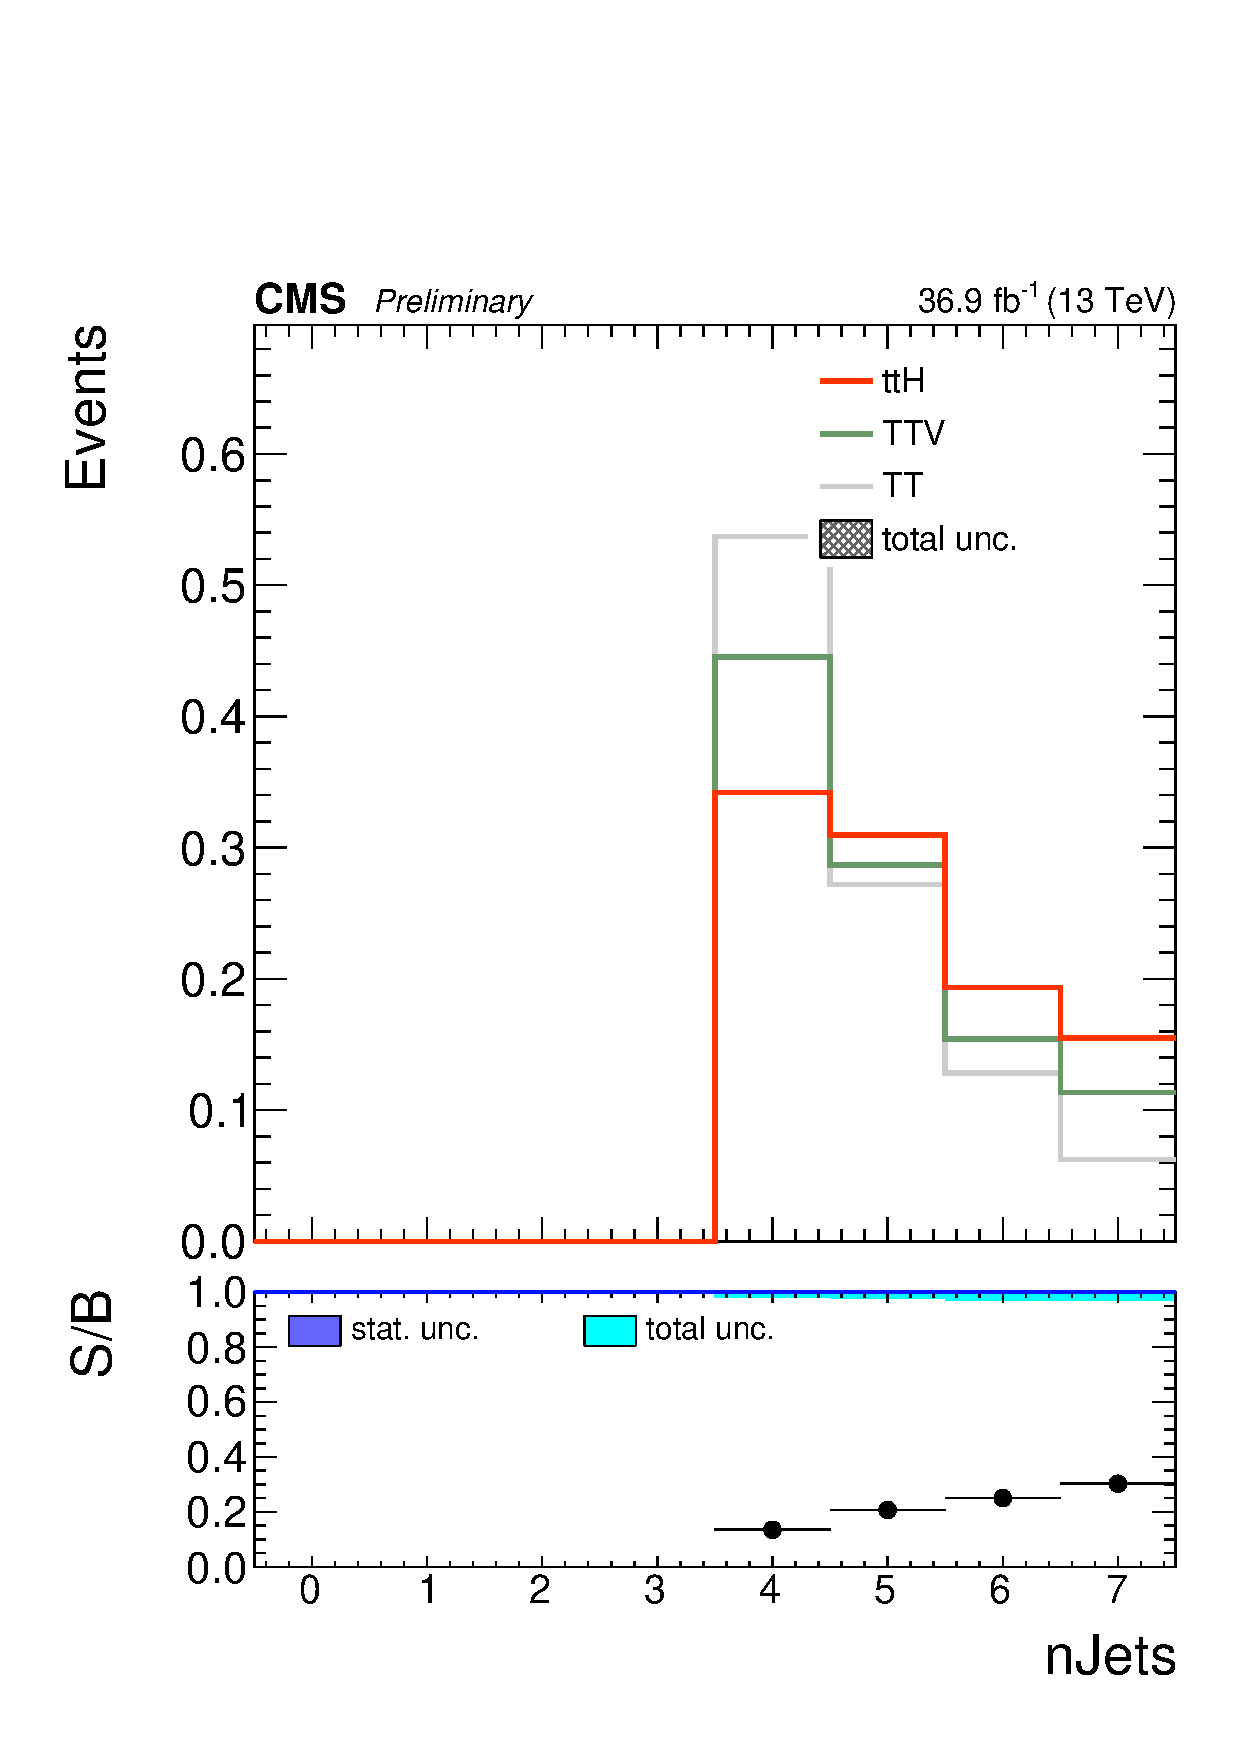
\includegraphics[width=0.49\textwidth]{ch9_figs/kinMVA_input_numJets.pdf}\\
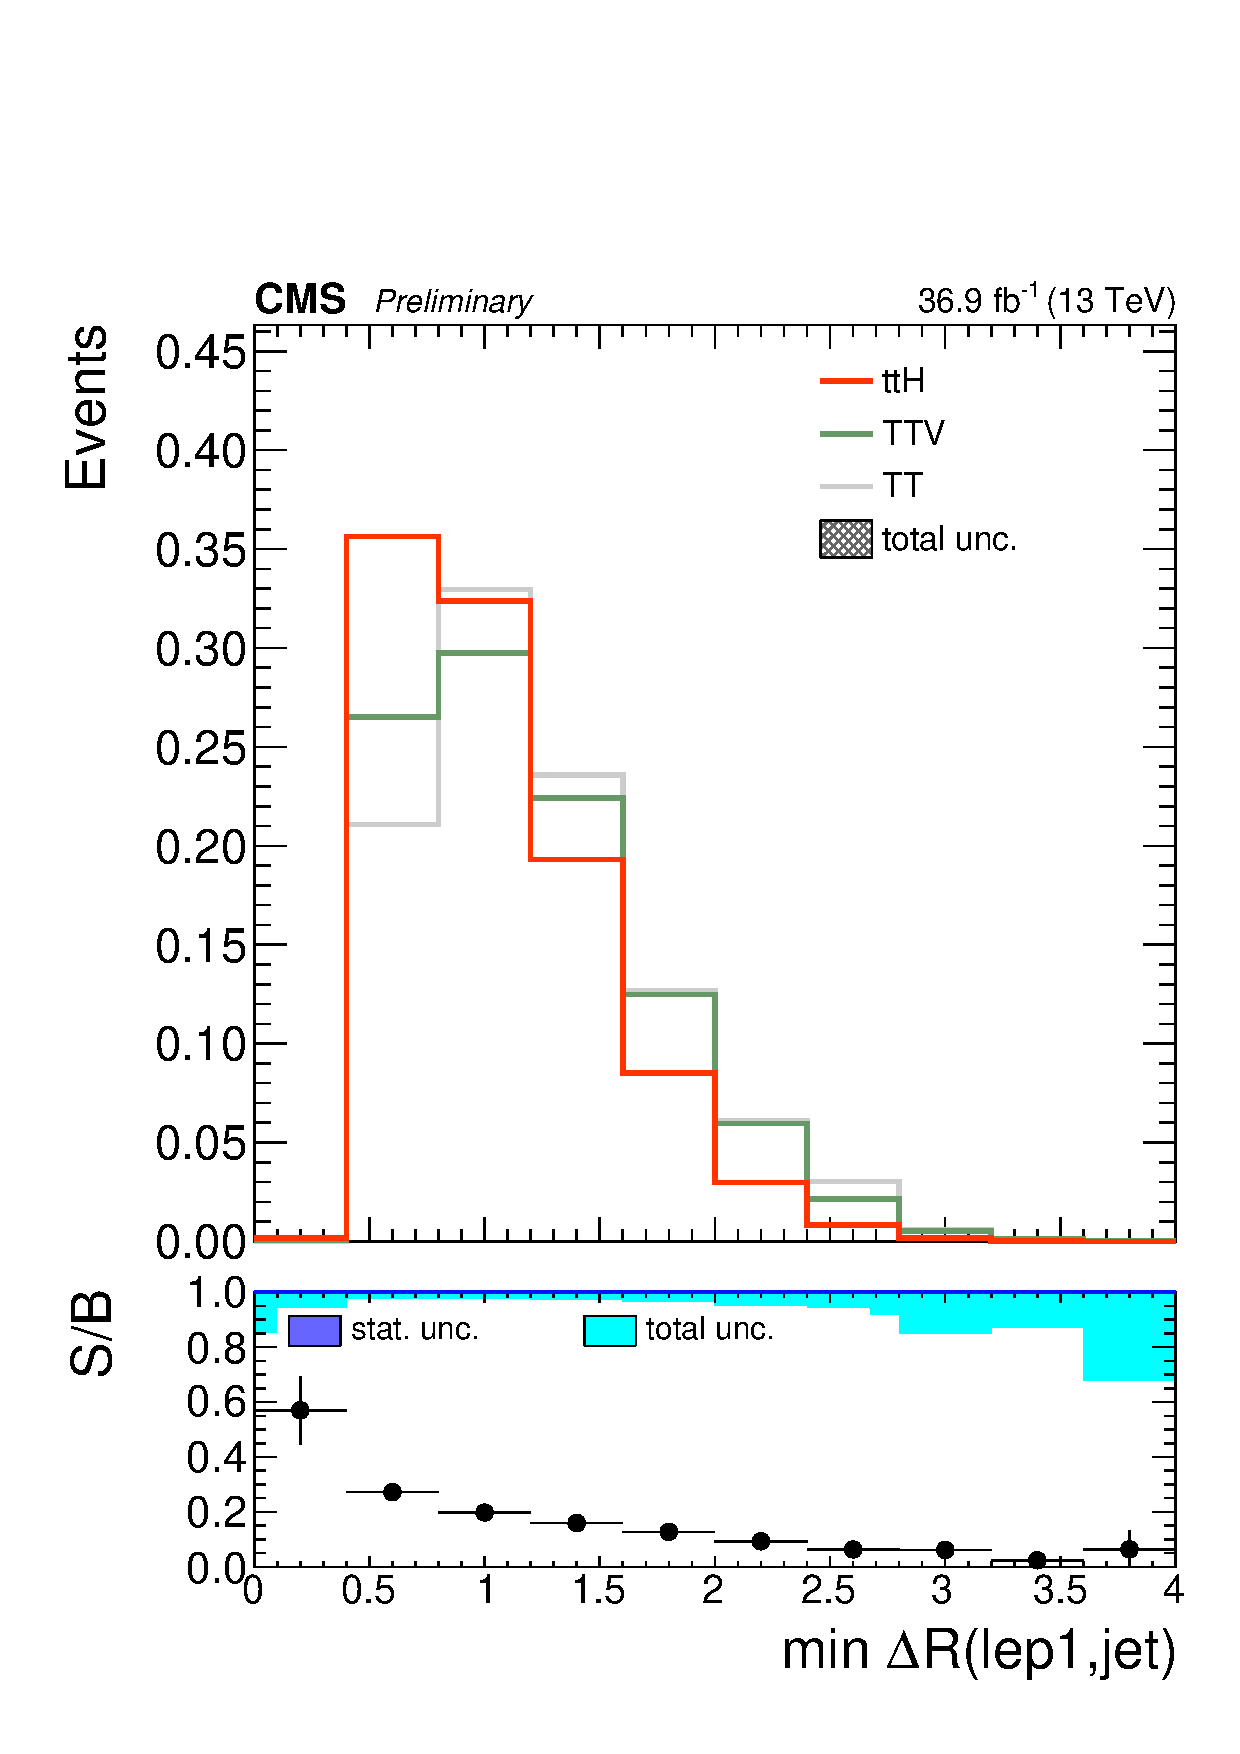
\includegraphics[width=0.49\textwidth]{ch9_figs/kinMVA_input_mindr_lep1_jet.pdf}
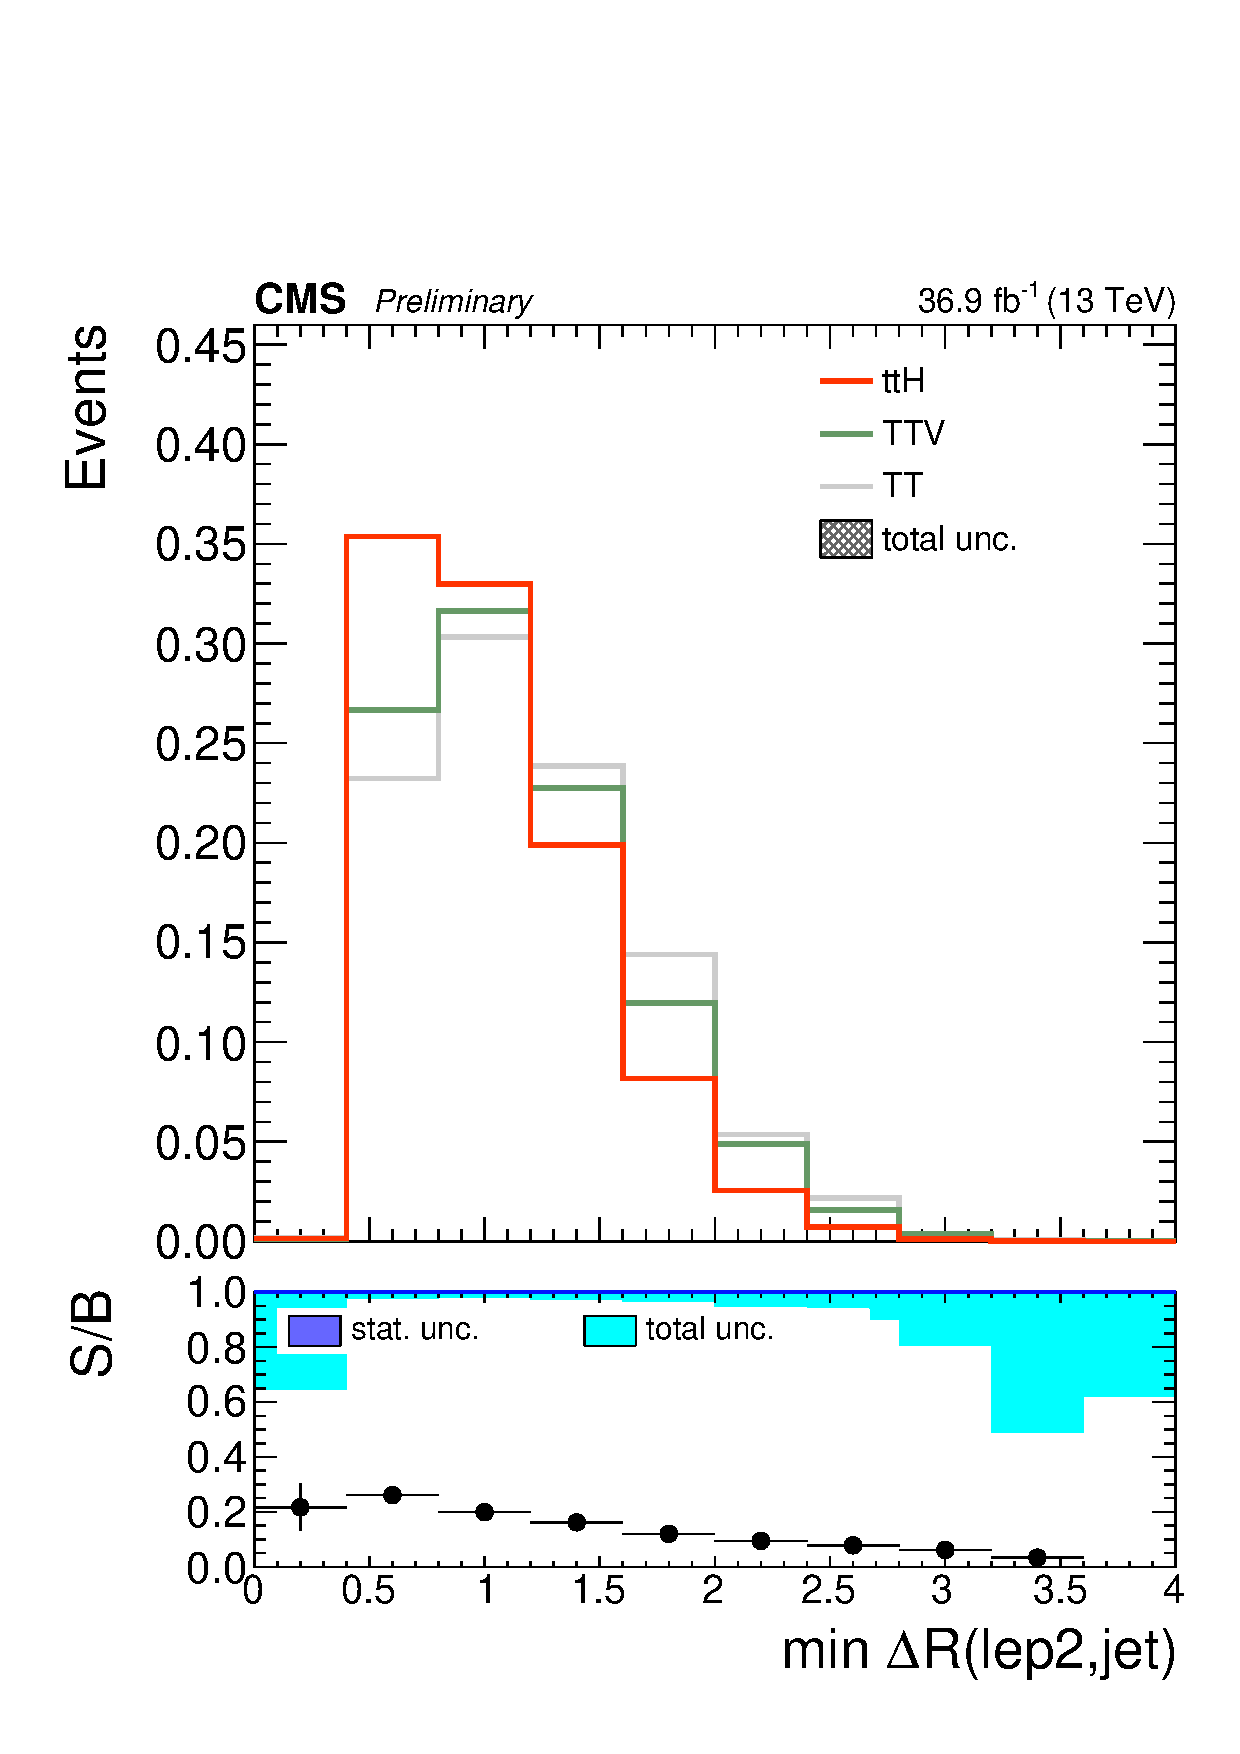
\includegraphics[width=0.49\textwidth]{ch9_figs/kinMVA_input_mindr_lep2_jet.pdf}
\caption[Signal extraction BDT input variables]{Separtion power among various backgrounds for BDT input variables}
\label{fig:inputs1}
\end{figure}

\begin{figure}[htp]
\centering
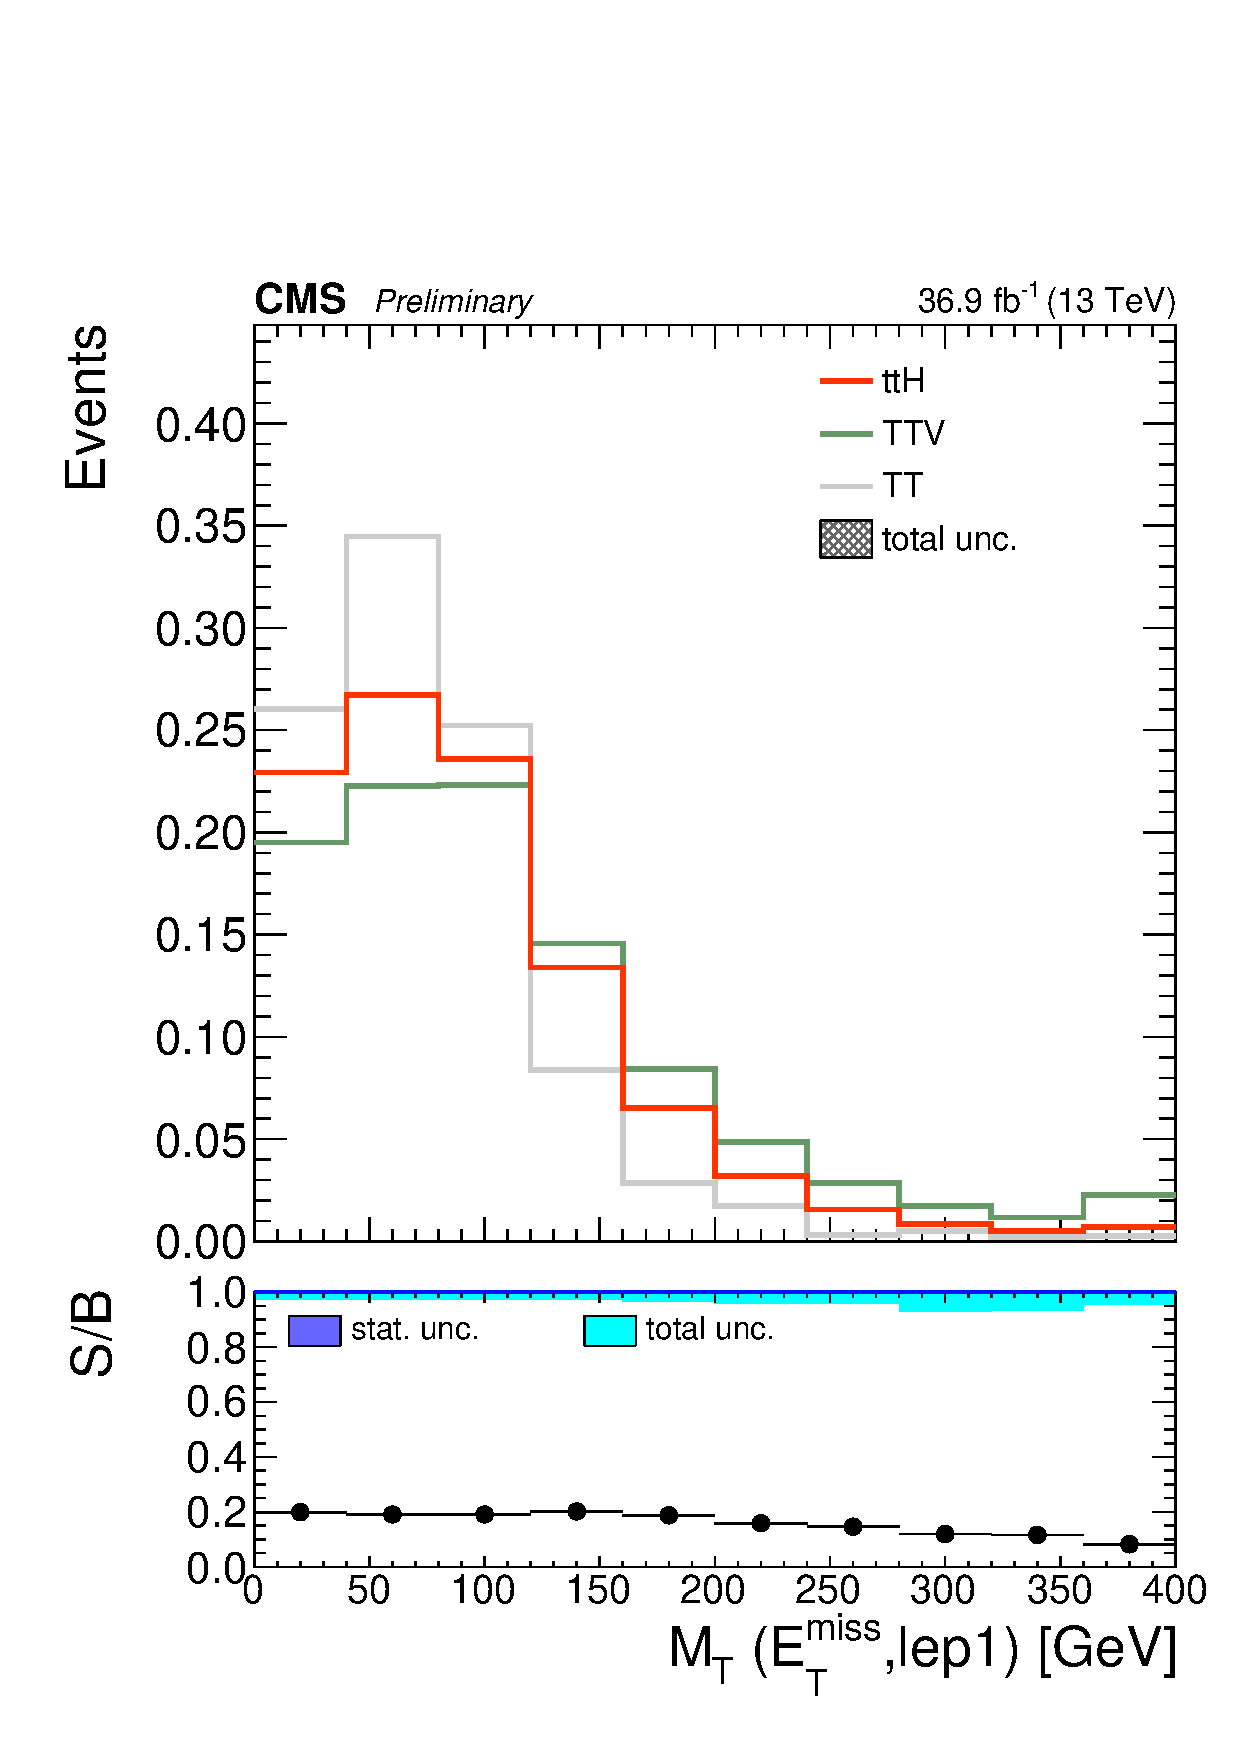
\includegraphics[width=0.49\textwidth]{ch9_figs/kinMVA_input_MT_met_lep1.pdf}
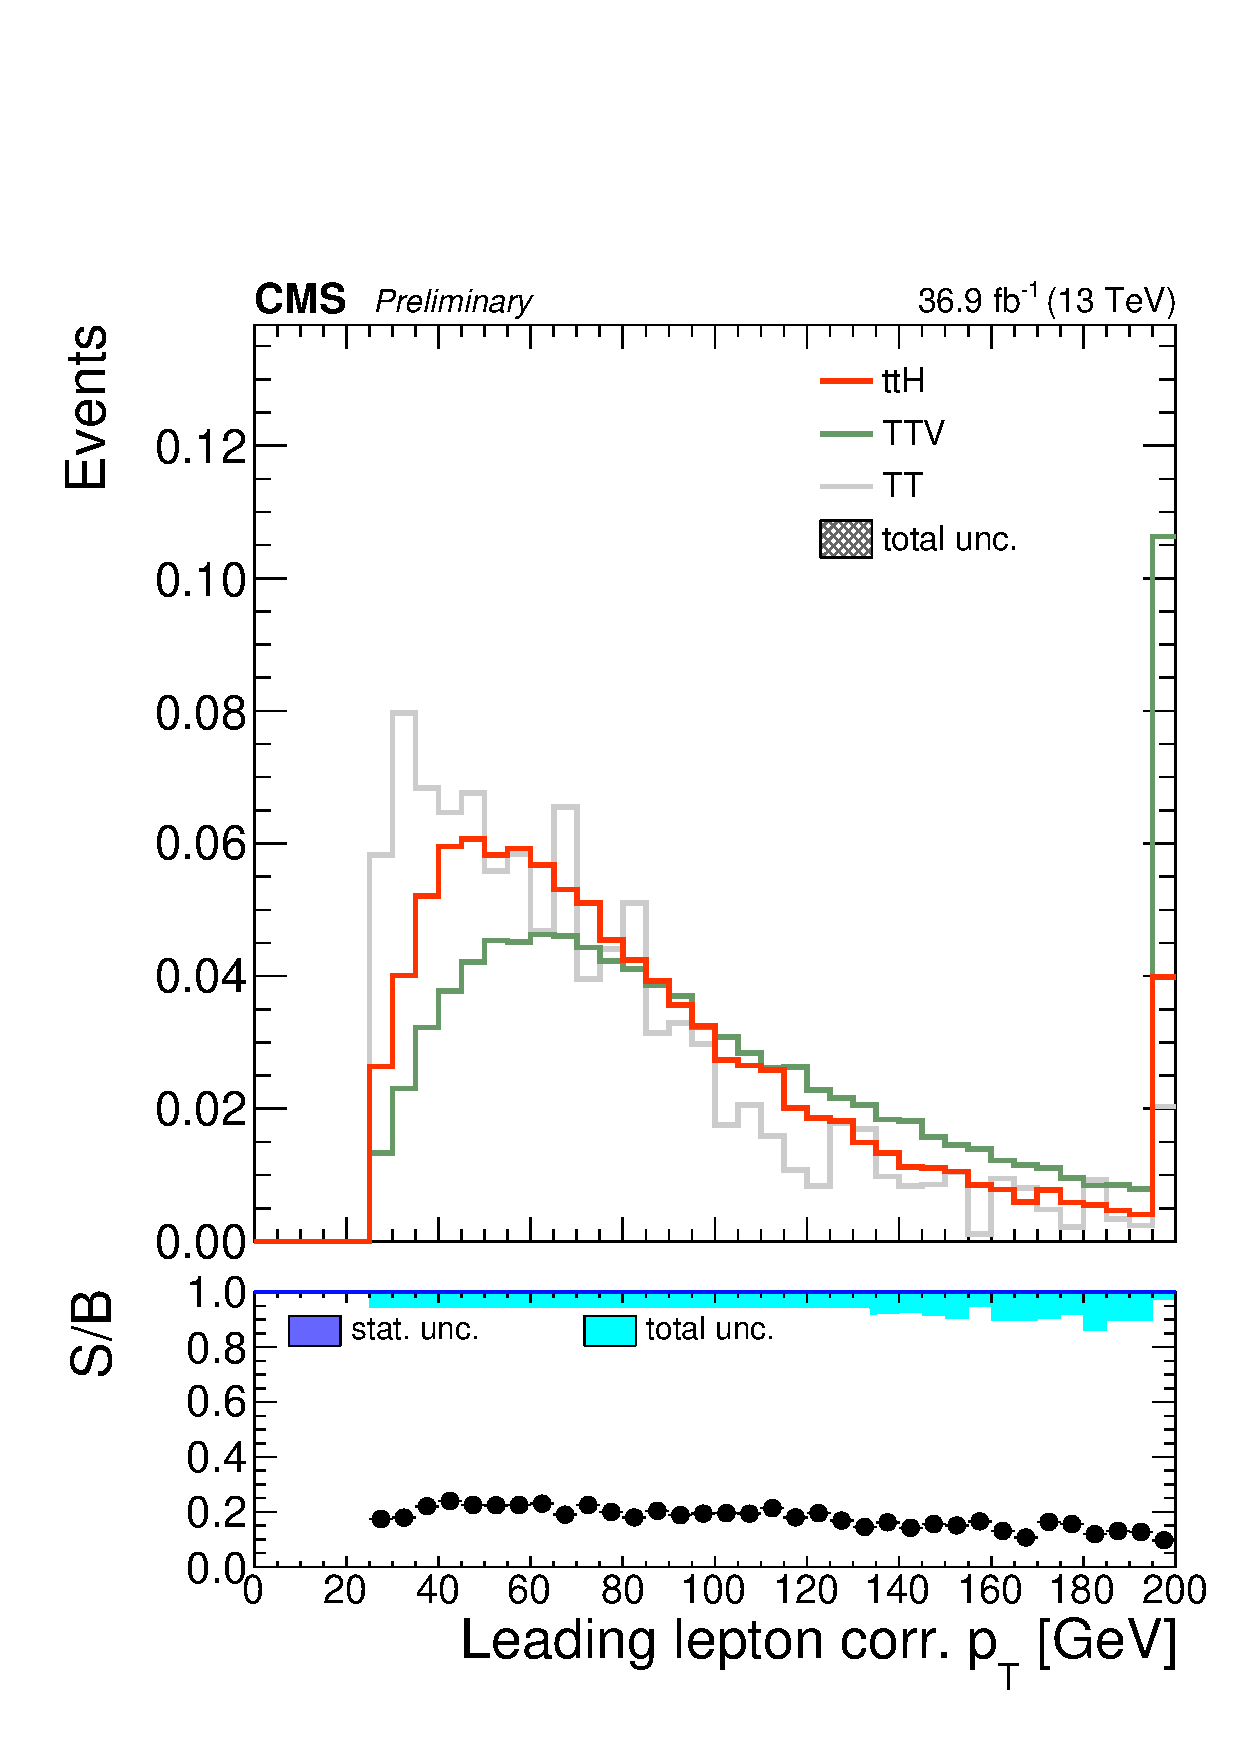
\includegraphics[width=0.49\textwidth]{ch9_figs/kinMVA_input_LepGood0_conePt.pdf}\\
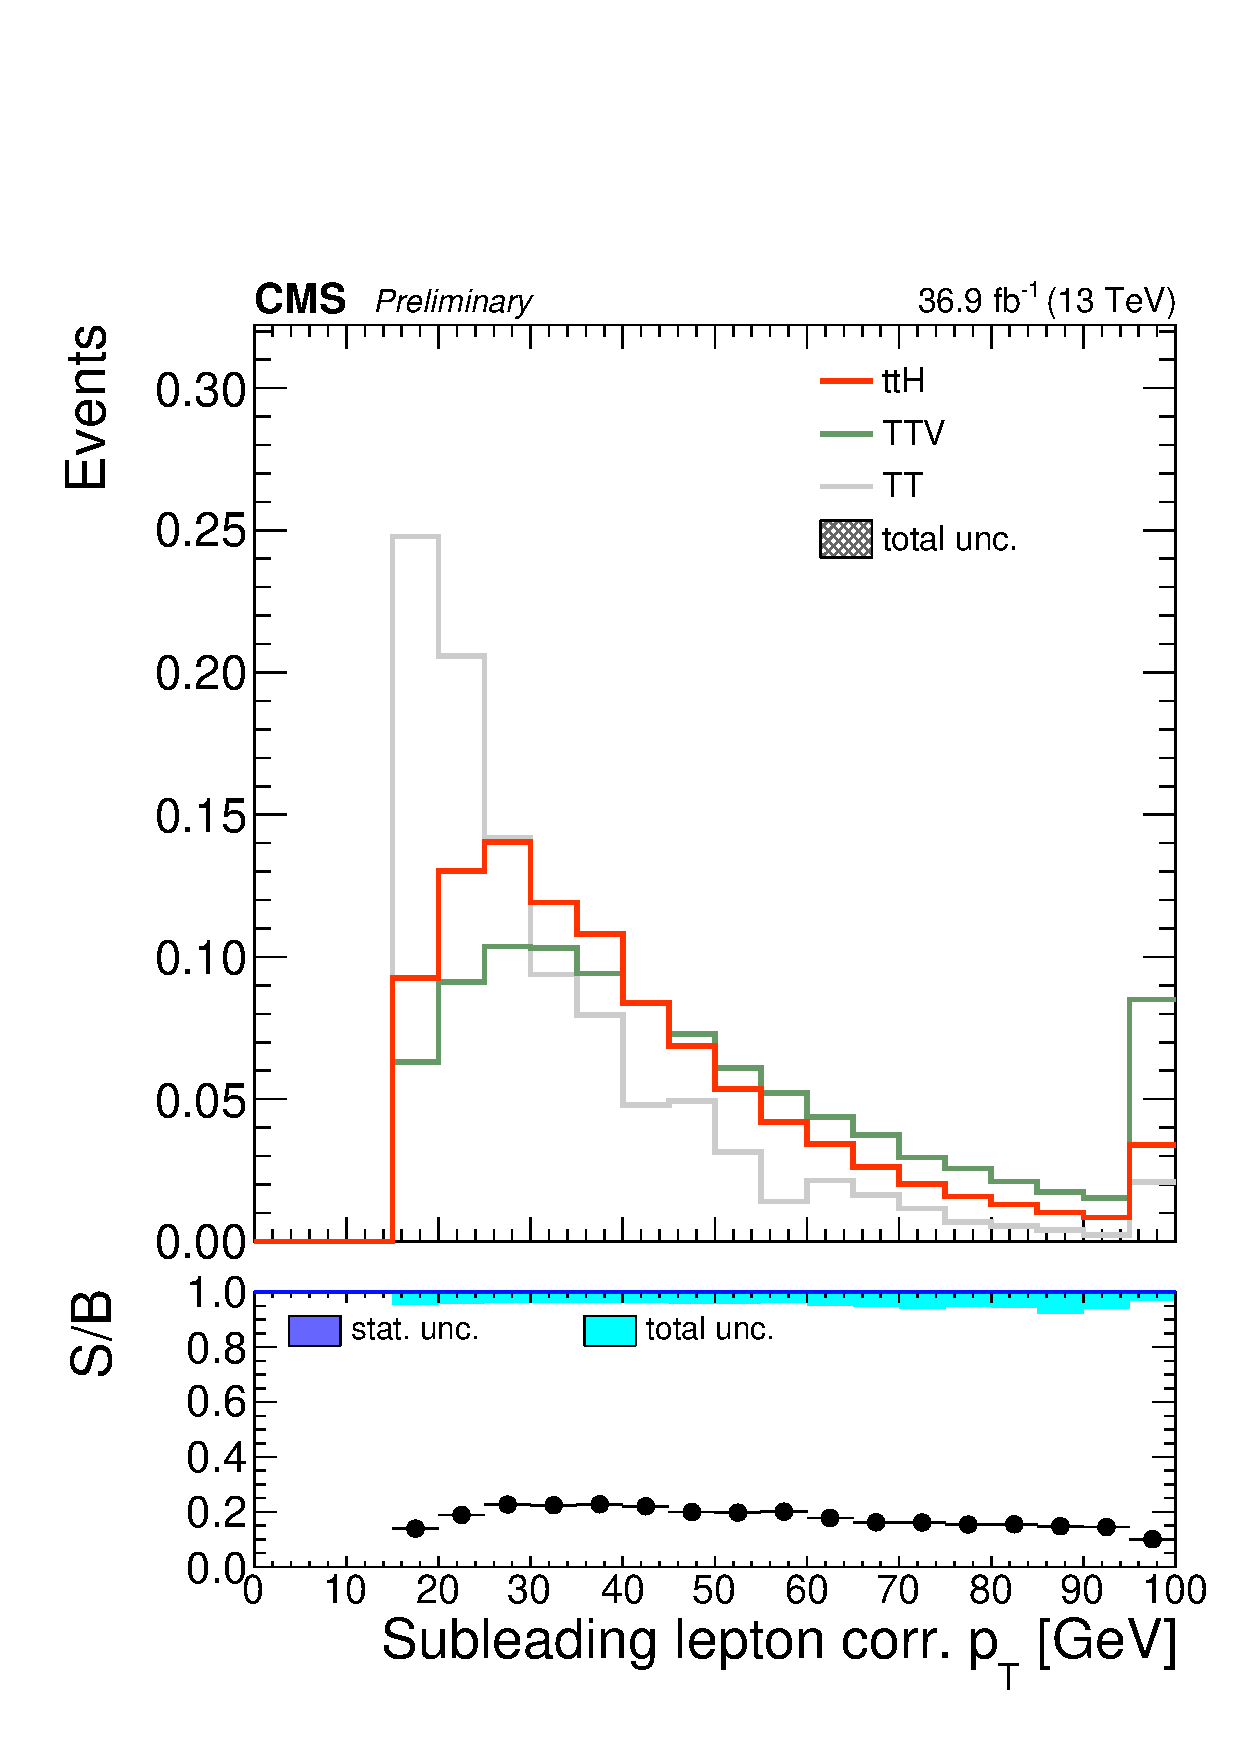
\includegraphics[width=0.49\textwidth]{ch9_figs/kinMVA_input_LepGood1_conePt.pdf}
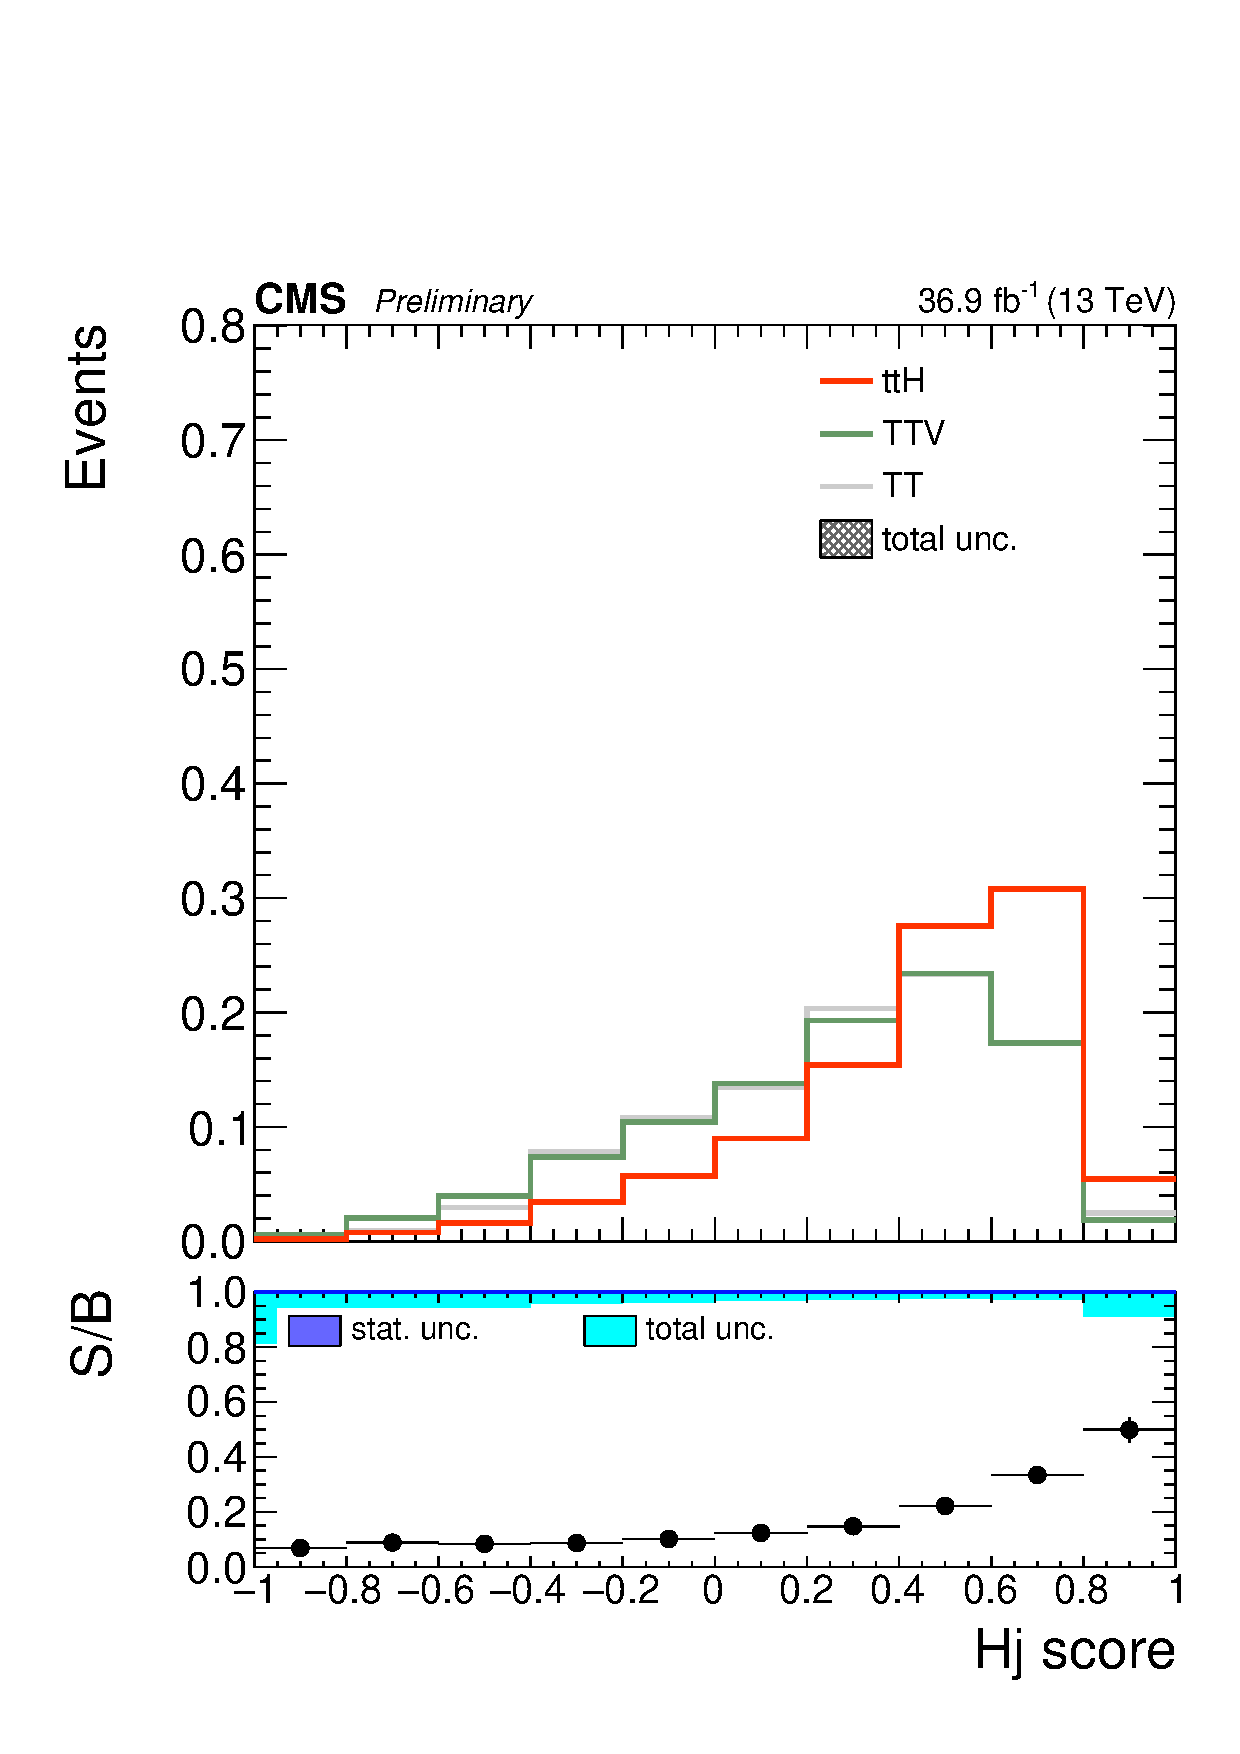
\includegraphics[width=0.49\textwidth]{ch9_figs/kinMVA_input_BDTv8_eventReco_Hj_score.pdf}
\caption[Signal extraction BDT input variables]{Separtion power among various backgrounds for BDT input variables}
\label{fig:inputs2}
\end{figure}

\begin{figure}[htp]
\centering
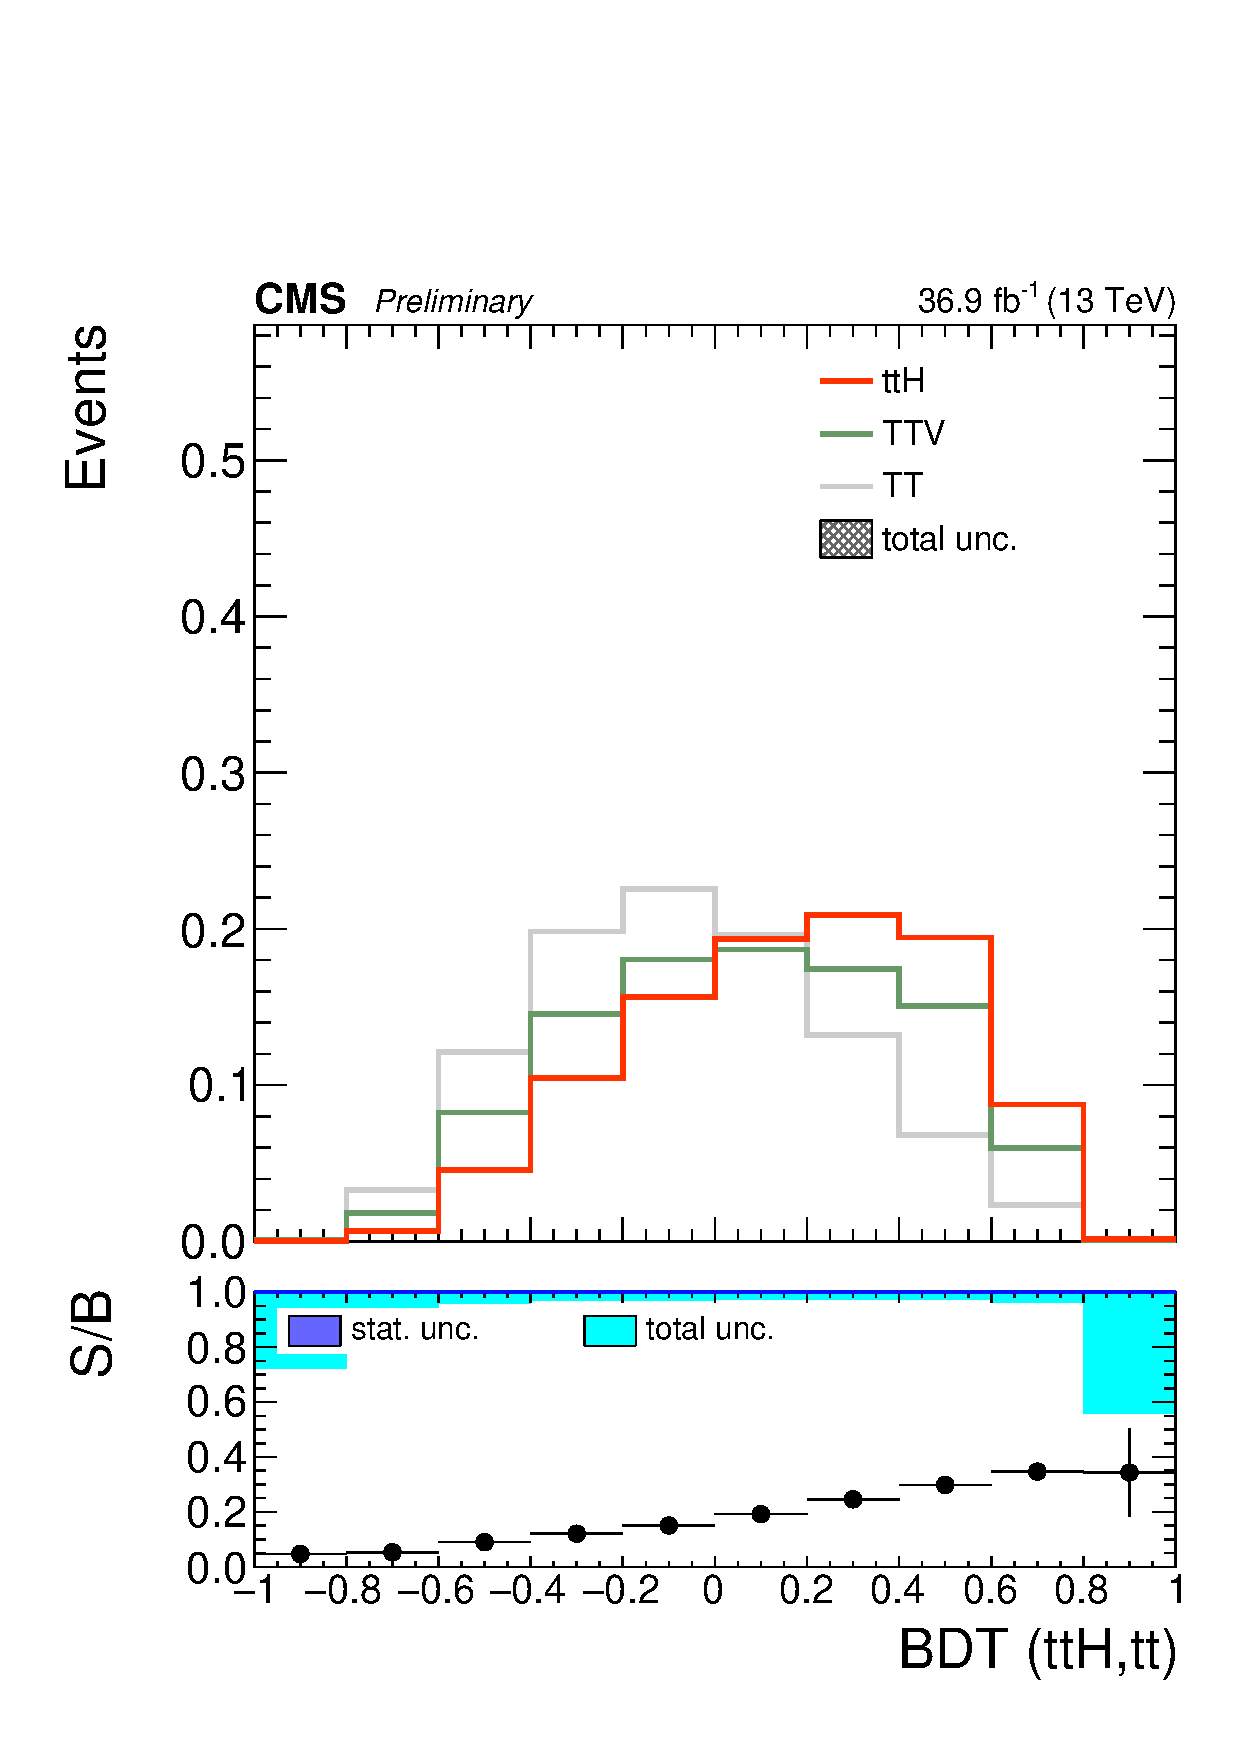
\includegraphics[width=0.49\textwidth]{ch9_figs/kinMVA_2lss_ttbar.pdf}
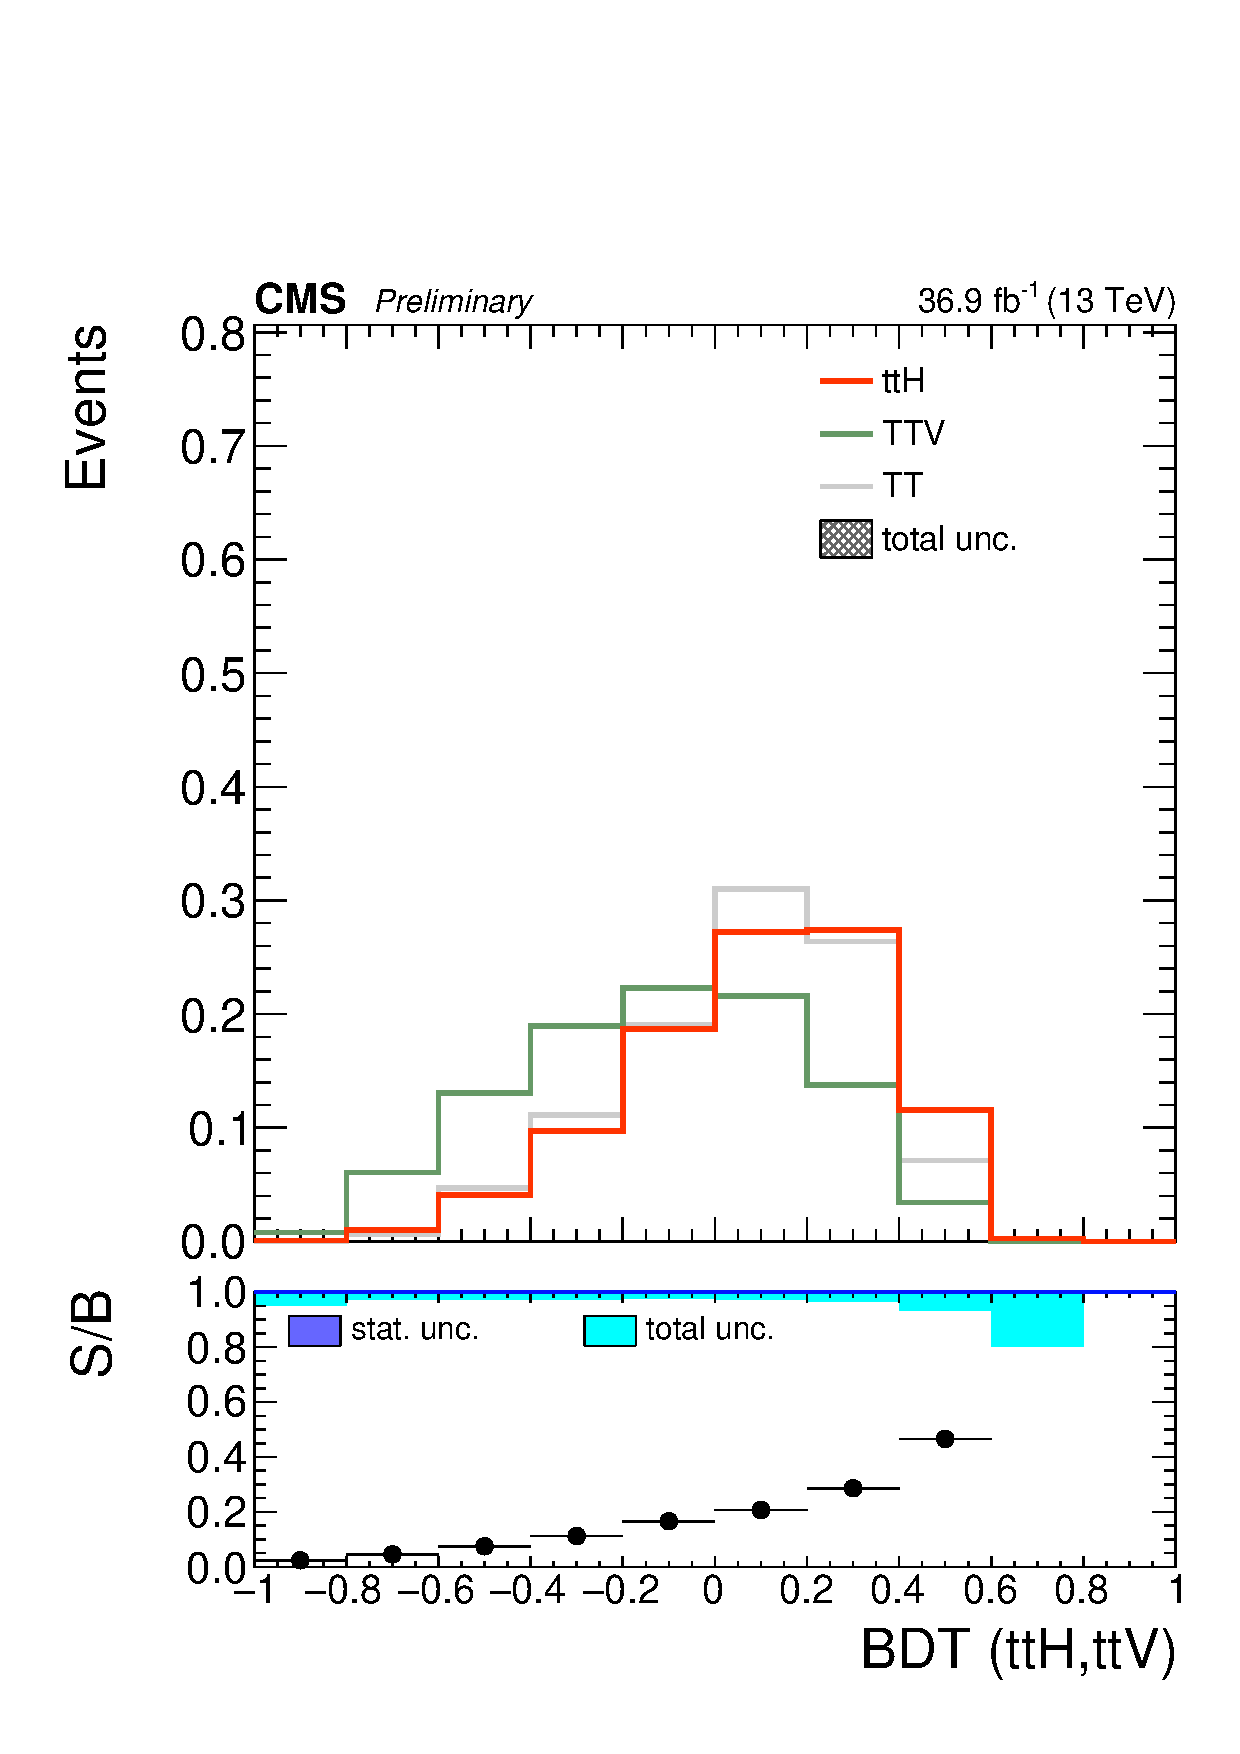
\includegraphics[width=0.49\textwidth]{ch9_figs/kinMVA_2lss_ttV.pdf}\\
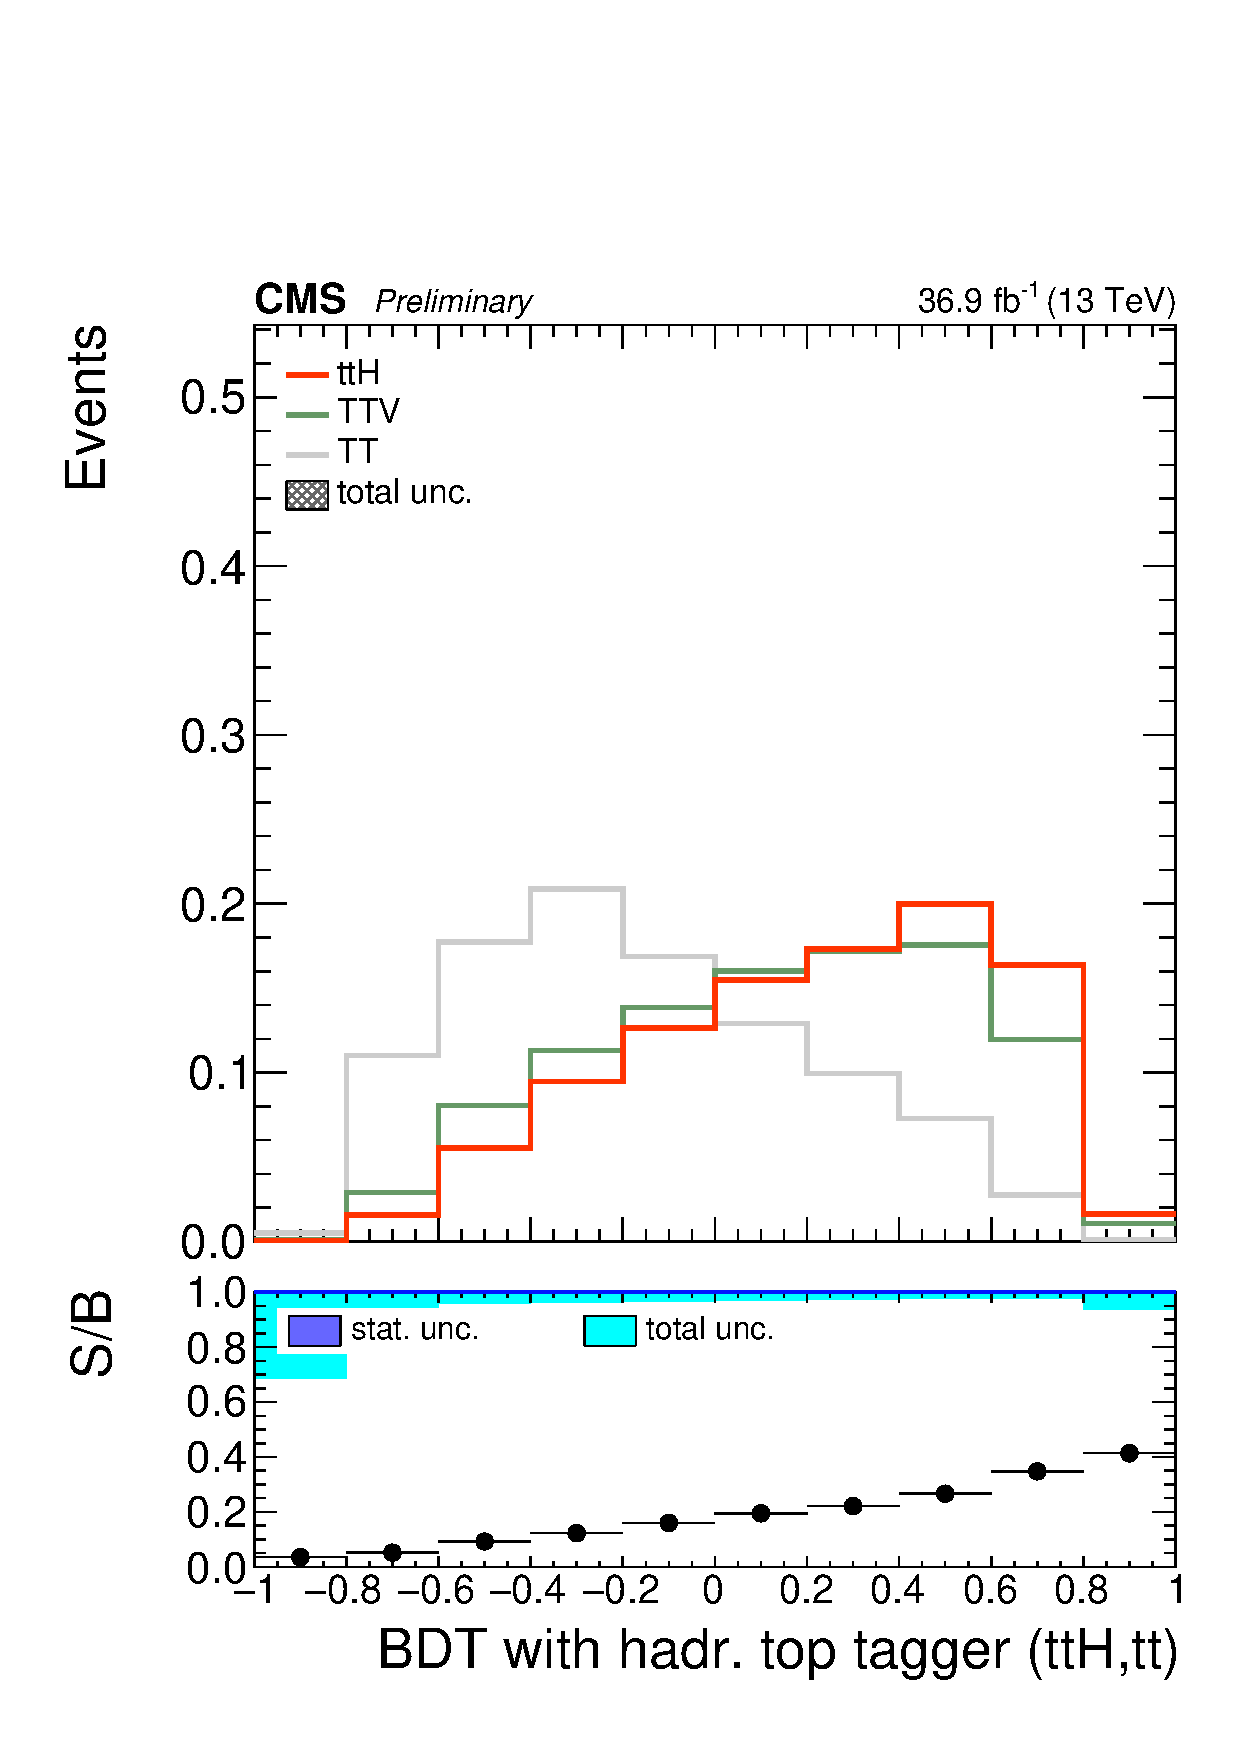
\includegraphics[width=0.49\textwidth]{ch9_figs/kinMVA_2lss_ttbar_withBDTv8.pdf}
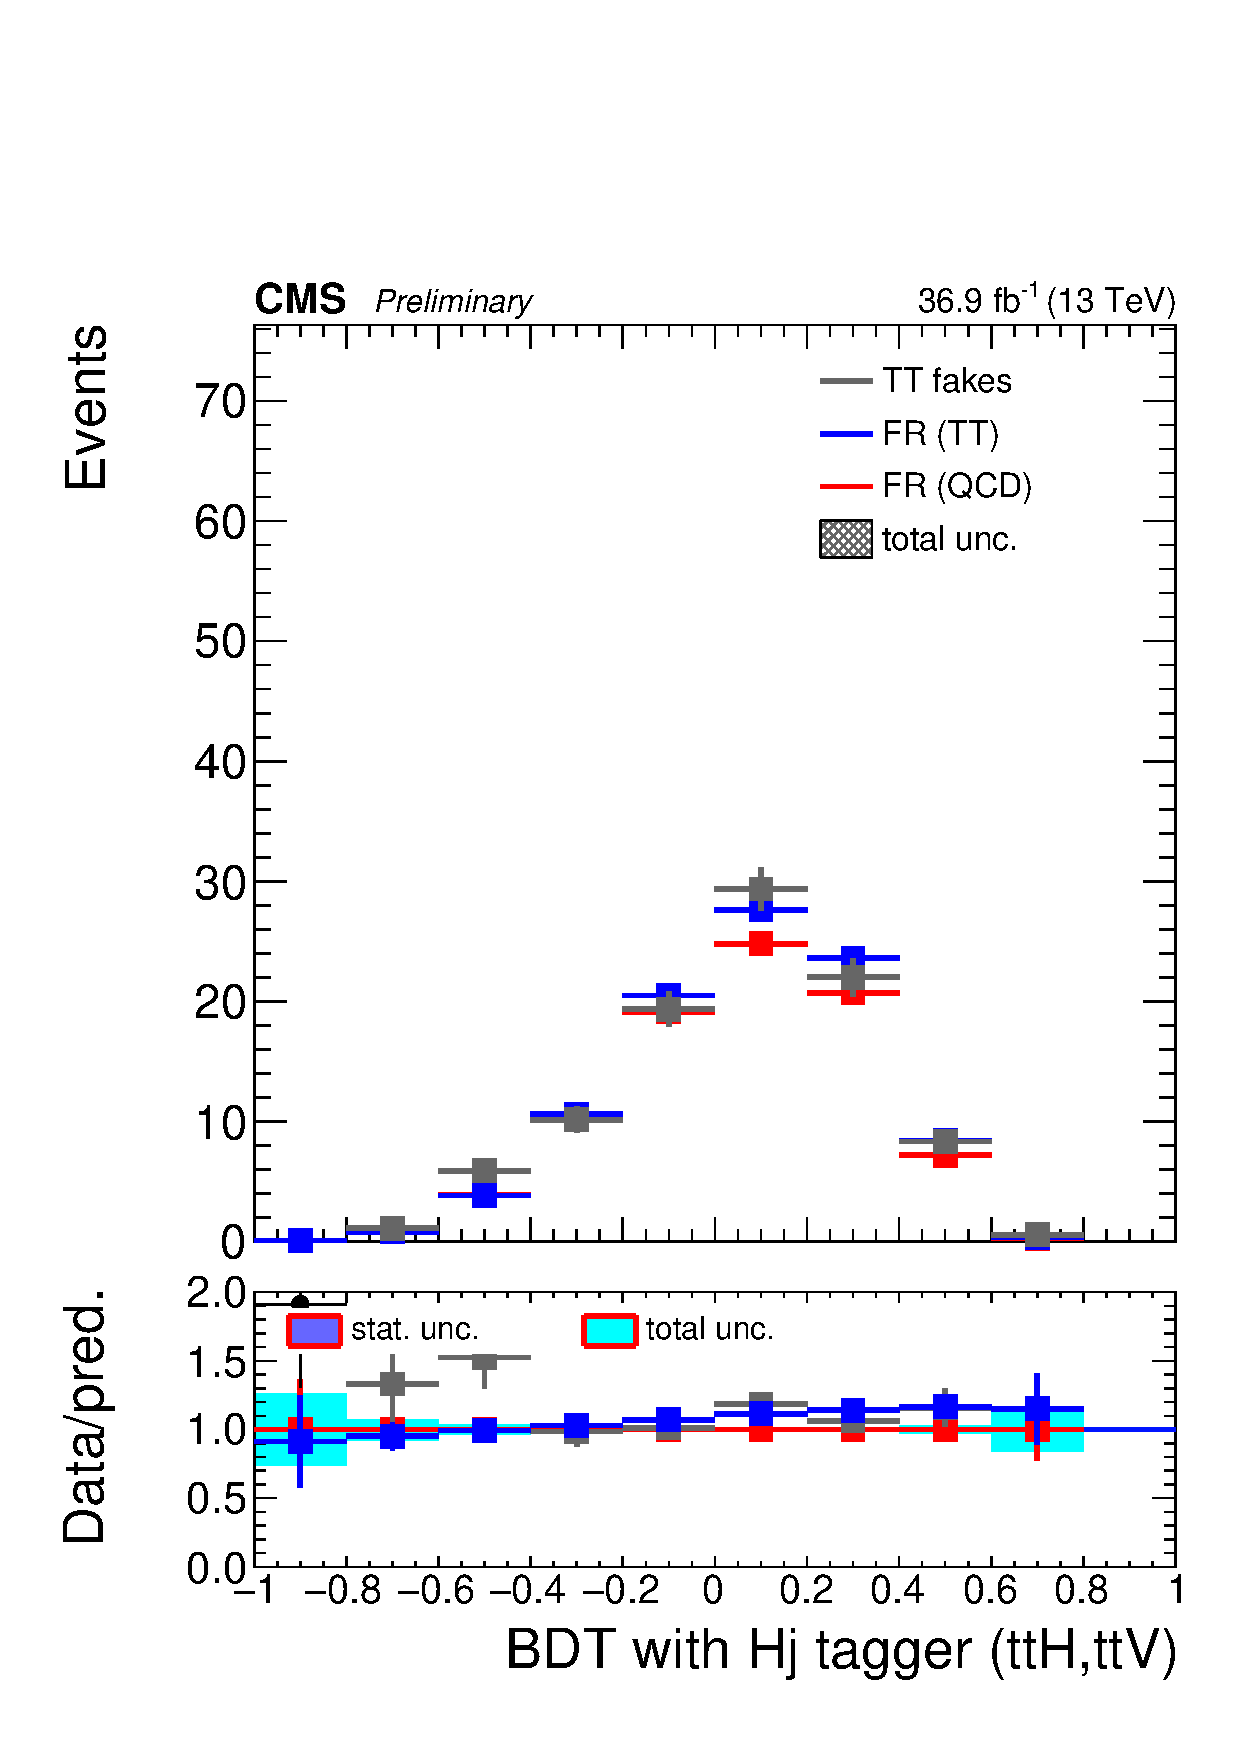
\includegraphics[width=0.49\textwidth]{ch9_figs/kinMVA_2lss_ttV_withHj.pdf}
\caption[BDT output scores with and without reconstruction inputs]{The BDT output scores without the reconstruction inputs (top) and with (bottom).}
\label{fig:inputs3}
\end{figure}

\subsection{Hadronic Top Reconstruction}
The reconstruction of the hadronic top decay is performed with a BDT. The objective is to correctly match
each selected jet and lepton to a final state particle in a $t\bar{t}H$ event, then
use the BDT response and other variables from the reconstruction to discriminate
against events without a hadronic top.     

Event reconstruction targets the 2lss category, specifically where the Higgs decays
to $W$ bosons. In the 2lss category, this means that one lepton originates from the
top system, and the other from the Higgs. For the jets, one of the
$W$ bosons from the Higgs decays hadronically, one of the top quarks decays
hadronically, producing a total of two b-jets, and four light-flavor jets
from the hadronic $W$ decays.   

{\bfseries Training}

The event reconstruction BDT is trained using the $t\bar{t}H$ monte-carlo powheg
signal sample described previously. 

The signal is correctly matched $t\bar{t}H$ events, which pass the 2lss selection.
Because the 2lss event selection requires at least four jets, the vast majority of signal
events used for training are only partially reconstructed, since a full reconstruction
necessitates six matched jets. Because so few events can be fully reconstructed, we must
consider partial reconstructions for events that have fewer than six matched jets.
The strategy for this is to use 'null' jets whose four-vectors are set to zero to
substitute missing jets in the event. Finally we require the signal events to have two
correctly matched selected leptons, and at least four correctly matched selected jets.

The background consists of all jet and lepton permutations of incorrectly matched
$t\bar{t}$ events. For the background, the null jets are added according to the
jet multiiplicity. For events with seven or fewer selected jets, three null jets are
added, for events with eight selected jets, two null jets are added, and one null jet
is added for events with greater than eight selected jets. To reduce the computation
time and improve performance,
several cuts are applied at each permutation to remove unlikely reconstructions.
These cuts include applying the b-tag requirement on the two jets being considered
as b-jets (1 b-tight, 2 b-loose) described earlier, requiring that no
reconstructed $W$ have a mass greater than 120 GeV, requiring the leptonic top mass
be less than 180 GeV, and requiring 
the hadronic top mass be less than 220 GeV. Additionally, we ignore permutations
arising from swapping two light flavor jets from the same $W$ boson, as the reconstruction is
identical. 

The BDT uses eight input variables, consisting of the CSV of the b-jets from the top
system, the transverse
momentum of the reconstructed hadronic top, the mass of the reconstructed hadronic top,
the mass of the $W$ originating from the hadronic top, the transverse momentum ratio
of lepton from the Higgs with the lepton from the top, and the solid angles between
the lepton from the top and
each b-jet from the top system, and between the lepton from the Higgs.
This approach focuses on the hadronic top decay, as the other aspects of the event
are more difficult to reconstruct due to the missing energy from the neutrinos. 

{\bfseries Evaluation}

The event reconstruction BDT is evaluated by iterating over all possible lepton and jet
permutations, and selecting the highest scoring permutation as the reconstruction for
each event. For the evaluation and usage, the null jet prescription and permutation
cuts used are identical to the background training.
The reconstruction is designed identify events that have a hadronic top present and thus offers
some discrimination against the semi-leptonic $t\bar{t}$ background, shown below in
Figure~\ref{reconstruction:outputVars}.

%% \begin{figure}[htb]
%%  \centering
%%    \includegraphics[width=0.4\textwidth]{plots_reconstruction/had_top_mass.png}
%%    \includegraphics[width=0.4\textwidth]{plots_reconstruction/had_top_pt.png}\\
%%    \includegraphics[width=0.4\textwidth]{plots_reconstruction/bdt_score.png}
%%    \caption{Best BDT score and associated quantities from hadronic top reconstruction.}
%%   \label{reconstruction:outputVars}
%% \end{figure}

\subsection{Higgs Jet Tagging}
The Higgs Jet (HJ) tagger is a BDT aimed specifically at identifying hadronic jets originating from the W bosons in \tth, H$\rightarrow$WW decays consistent
with the \tth diagram in Figure~\ref{fig:intro_feyn}. This decay topology is the most common of all \tth decays in the $2lss$ channel. This final state
consists of 2 b-quark jets, 4 hadronic (light flavor) jets, 2 same-sign leptons, and missing energy due to neutrinos. The signal region selection described
in Chapter~\ref{chap:event_selection} does not require all of these objects to be present, as some or many are often out of the acceptance. This means that
the jets from the Higgs decay could be missing entirely from the event.

The HJ tagger addresses both the complicated jet combinatorics associated with this final state, but also the reality that not all jets originating
from the Higgs are selected. The HJ tagger is an object-level discriminator that exploits jet kinematics and identification variables to estimate the likelihood
of a jet originating from the Higgs. Similar to the hadronic top reconstruction method, the HJ tagger calculates scores for every jet in each event, selecting
the highest score as the output. To boost performance and simplify the combinatorics associated with tagging, the hadronic top tagger is first run,
and the jets selected as being assocaited with the hadronic top are removed from further consideration by the HJ tagger.
The HJ tagger is primarily aimed at selected jets from W decays (from the Higgs) and is used as a discriminating varible against both the \ttw and \ttz backgrounds.
Both of these
backgrounds are very likely to contain most or all of the hadronic top decay products, namely a b-tagged jet and two light flavor jets. The two light flavor jets from
the W in the hadronic top decay look kinematically similar to the targeted jets from the W from the Higgs, creating a potential for Higgs jet mis-tagging. This is
especially true when the b-jet is missing. The hadronic top tagger idenifies these jets and they are removed from consideration by the HJ tagger.

The HJ tagger is trained on \tth and \ttv MC. The signal training events require the reco-level objects passing the selection to be matched to a generator-level parton
originating from the H$\rightarrow$WW$\rightarrow l\nu~l\nu$ process. The background selection requires \ttv events in the signal region.  
The input variables include:
\begin{itemize}
\item the minimum angular separation between the jet and one of the two leptons
\item the maximum angular separation between the jet and one of the two leptons
\item the jet transverse momenta
\item the jet b-tag discriminator (CSVv2)
\item the jet quark-gluon discriminator (qgid)
\end{itemize}

\noindent The qgid varible is a BDT designed to discriminate jets originating from light flavor quarks from jets originating from gluons. The performance and improvement due
to the HJ tagger input is seen in Figure~\ref{fig:hj_tagger}.

\begin{figure}[htp]
\centering
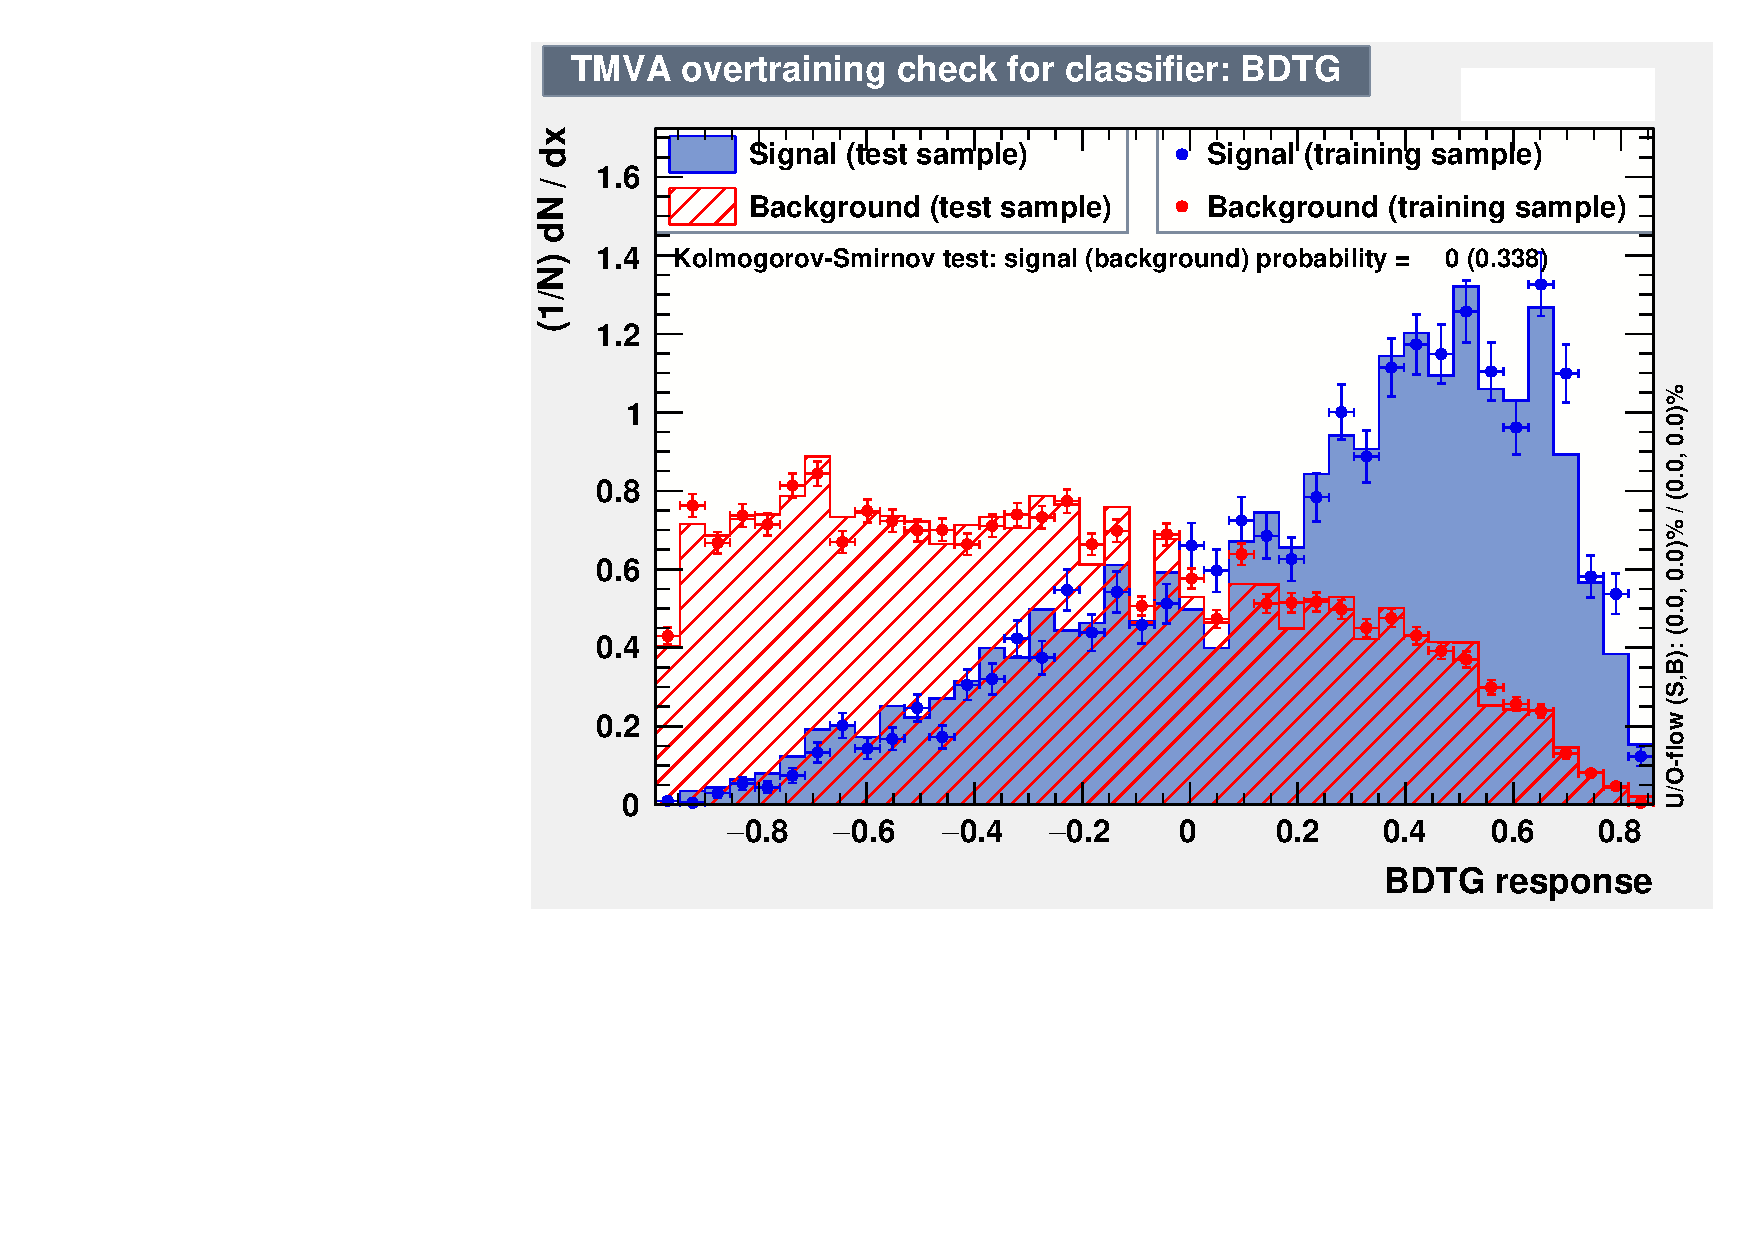
\includegraphics[width=0.49\textwidth]{ch9_figs/Jtagger_Ks.pdf}
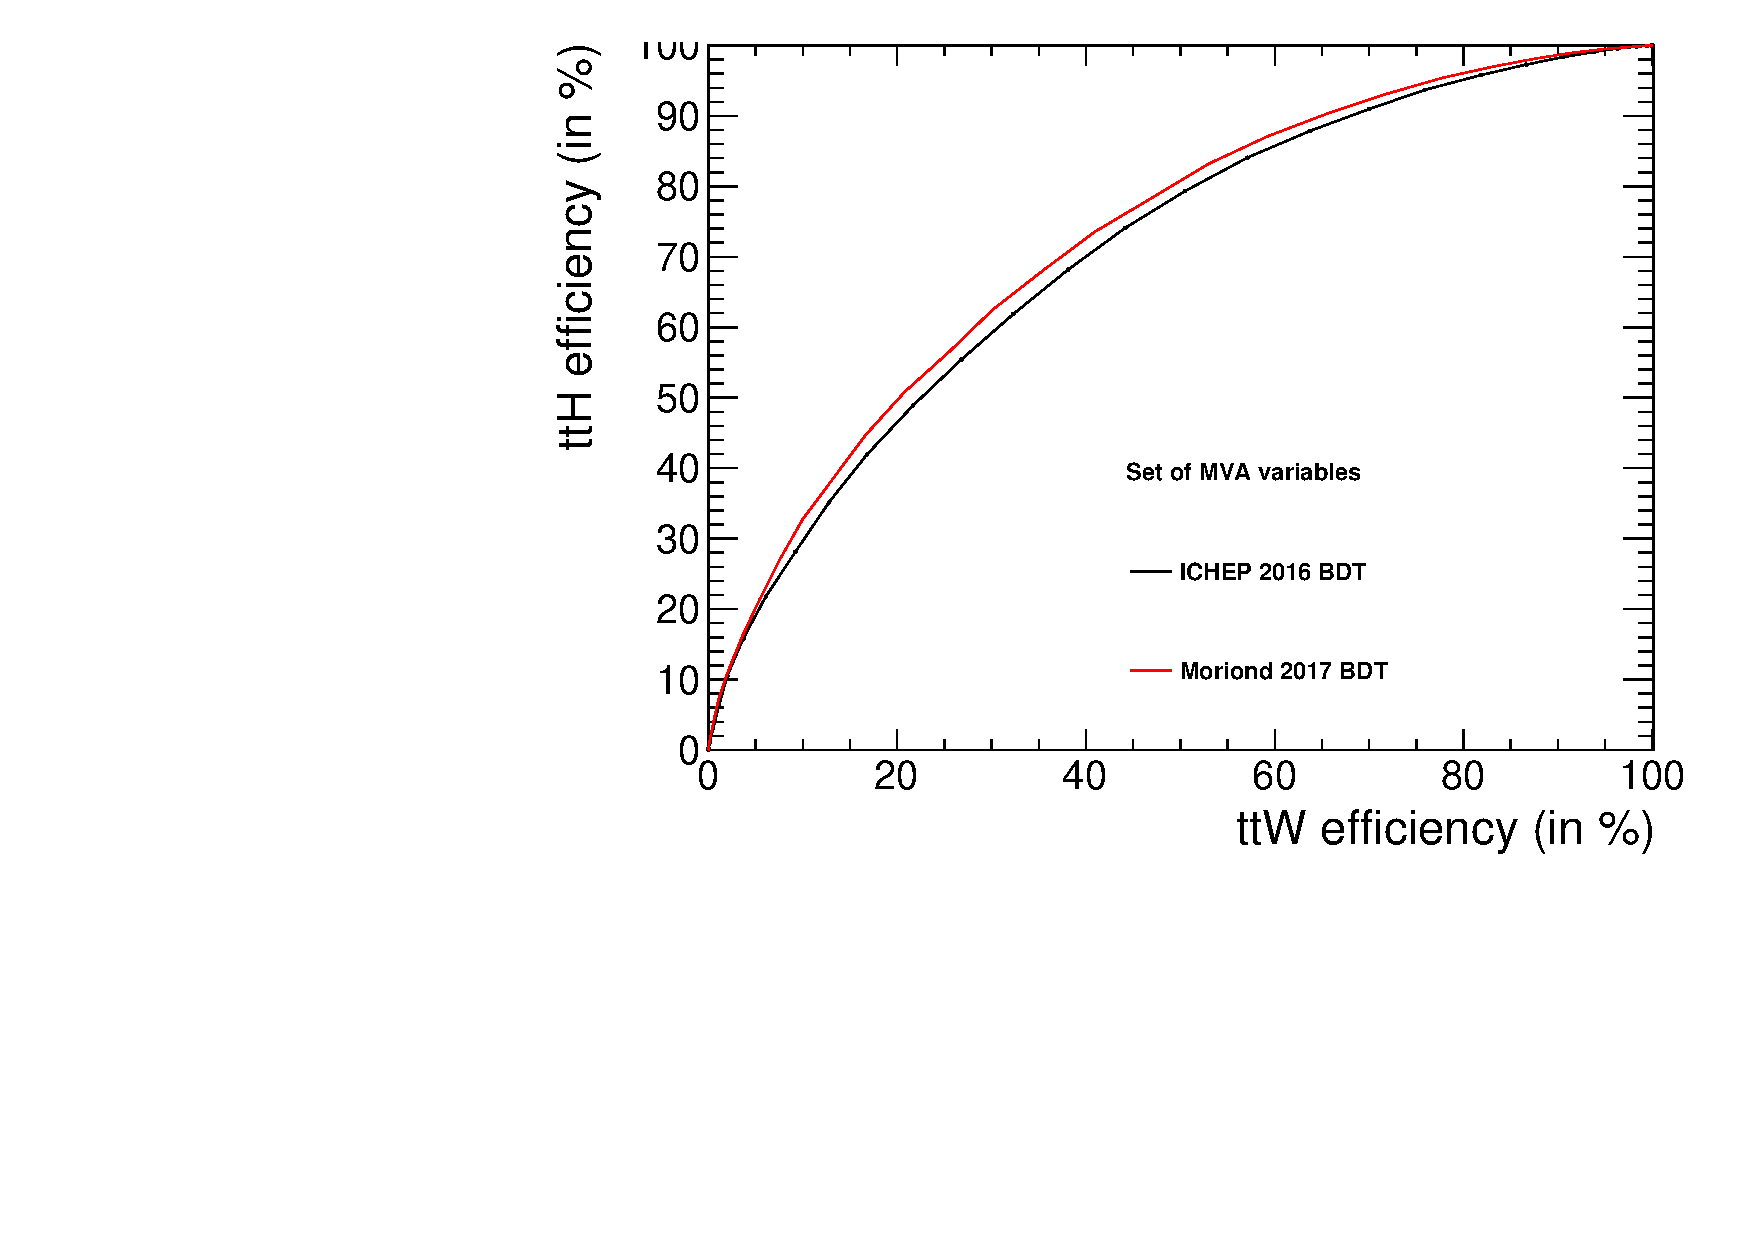
\includegraphics[width=0.49\textwidth]{ch9_figs/Roc_Comparison_18Feb.pdf}
\caption[Performance improvement from the HJ tagger and hadronic top removal]{Separation power of HJ output on the training samples (right) and performance improvements with respect to the 2016 version of this analysis obtained with the HJ
tagger input with hadronic top removal (left).}
\label{fig:hj_tagger}
\end{figure}

\section{Binning}
Binning the two-dimensional shape resulting from plotting each BDT on a separate axis is very non-trivial, since overlaying the shapes across signal and backgrounds is not possible. The binning method must optimally partition the space to isolate
signal from background, while simultaneously maintaining populated bins that don't suffer from low statistics. The best approach was 

\begin{figure}[htp]
\centering
\includegraphics[width=0.49\textwidth]{ch9_figs/}\\
\includegraphics[width=0.49\textwidth]{ch9_figs/}
\includegraphics[width=0.49\textwidth]{ch9_figs/}
\caption[Two dimensional BDT output shapes of signal and backgrounds]{}
\label{fig:2d_shapes}
\end{figure}


\section{Subcategorization}


